\documentclass[UKenglish]{article}
\usepackage[utf8]{inputenc}           %% ... or latin1
\usepackage[T1]{fontenc,url}
\urlstyle{sf}
\usepackage{babel,textcomp,csquotes,DUO/duomasterforside,varioref,graphicx}
\usepackage[backend=biber,style=numeric-comp,sorting=none]{biblatex}
\usepackage{amsmath,amssymb,amsfonts}
\usepackage{algorithmic}
\usepackage{textcomp}
\usepackage{xcolor}
\usepackage{textgreek}
\usepackage{float}
\usepackage{graphicx}
\usepackage{titlesec}
\usepackage{glossaries-extra}
\usepackage{verbatim}
\titleformat{\chapter}{\normalfont\huge}{\thechapter.}{20pt}{\huge}

\raggedbottom %%reduces the gaps between the paragraphs

\addbibresource{bibliography.bib}

% Abbreviations
\setabbreviationstyle[acronym]{long-short}
% \makeglossaries % Comment in when printing glossaries.
\usepackage{glossaries-extra}
\setabbreviationstyle[acronym]{long-short}


\newacronym{cnn}{CNN}{Convolutional Neural Network}
\newacronym{rnn}{RNN}{Recurrent Neural Network}
\newacronym{cpu}{CPU}{Central Processing Unit}
\newacronym{gpu}{GPU}{Graphics Processing Unit}
\newacronym{vqa}{VQA}{Visual Question Answering}
\newacronym{xai}{XAI}{Explainable Artificial Intelligence} % Should it be Explainable or eXplainable?
\newacronym{ai}{AI}{Artificial Intelligence}
\newacronym{ml}{ML}{Machine Learning}
\newacronym{shap}{SHAP}{SHapley Additive exPlanations}
\newacronym{lime}{LIME}{Local Interpretable Model-agnostic Explanations}
\newacronym{knn}{k-NN}{k-Nearest Neighbors}
\newacronym{gradcam}{Grad-CAM}{Gradient-weighted Class Activation Mapping}
\newacronym{flex}{FLEX}{Faithful Linguistic Explanations}
\newacronym{lstm}{LSTM}{Long Short-Term Memory}
\newacronym{sota}{SOTA}{State-of-the-Art}
\newacronym{nlp}{NLP}{Natural Language Processing}
\newacronym{bvlc}{BVLC}{The Berkeley Vision and Learning Center} % Developed Caffe together with BAIR
\newacronym{bair}{BAIR}{Berkeley AI Research} % Developed Caffe together with BVLC
\newacronym{svm}{SVM}{Support Vector Machines}
\newacronym{svd}{SVD}{Singular Value Decomposition}
\newacronym{pca}{PCA}{Principal Component Analysis}
\newacronym{imagenet}{ILSVRC}{ImageNet Large Scale Visual Recognition Challenge}
\newacronym{ann}{ANN}{Artificial Neural Network}
\newacronym{vit}{ViT}{Vision Transformer}
\newacronym{bert}{BERT}{Bidirectional Encoder Representations from Transformers}
\newacronym{bart}{BART}{Bidirectional Auto-Regressive Transformers}
\newacronym{gpt}{GPT}{Generative Pre-trained Transformer}
\newacronym{vram}{VRAM}{Video RAM}
\newacronym{lora}{LoRA}{Low-Rank Adaptation}
\newacronym{llama}{LLaMA}{Large Language Model Meta AI}
\newacronym{llm}{LLM}{Large Language Model}
\newacronym{roi}{ROI}{Region of Interest}
\newacronym{vgg}{VGG}{Visual Geometry Group}
\newacronym{cuda}{CUDA}{Compute Unified Device Architecture}
\newacronym{relu}{ReLU}{Rectified Linear Unit}
\newacronym{sdg}{SDG}{Stochastic Gradient Descent}

\begin{document}
    \title{Explaining images with locally faithful captions \\ \large Essay}     
    \author{Emil Christopher Gjøstøl Strømsvåg}
    \date{November 2022}
    \maketitle

%\frontmatter{}
\newpage
% Print Abbreviations
% \printglossary[type=\acronymtype,title={List of Acronyms}]
\tableofcontents{}
\newpage
%\listoffigures{}
%\listoftables{}

%\mainmatter{}

%\section{Abstract}
\label{sec:abstract}

\begin{comment}
The abstract is often the first text the reader looks at. Thus, it should be very well written, concise and to-the-point - with the focus of SELLING your work. It is therefore often written at the very end, when you have all details of your work. Usually, we recommend something like this: i) A sentence or three about the background of the challenge you are addressing, which then leads to your “problem statement” (written as just a sentence); ii) Some text describing what you have done in your research, what have you developed, etc.; iii) A small overview of your main results and conclusions - what are the main take-aways from your thesis.

Note also that the abstract is a teaser, and it should therefore not be too long: Fast to read, fast to get to the point. We often recommend keeping it on one page.
\end{comment}


% More complex models
With the increase in accuracy and usability of deep neural networks, there has been a big demand for using these neural networks in different domains to increase productivity, create new industries, and improve people's lives. 
However, these networks are often large and complex, which does not give insight into the prediction process done by the model. 
In order to make the models more functional and be able to improve them, humans need to understand how they reason. 

This thesis will explore image captioning systems that are locally faithful to the underlying method using gradient activations in the network combined with a language model trained on open-ended questions and answers. % Max one page
%\part{Introduction}

%\section{Problem and Application}
%\chapter{Problem and Application} % Three pages
\label{sec:2_problem_and_application}
\section{Problem and application}
% Intro to this chapter

The increasing use of \gls{ai} has led to significant advances in various areas. However, understanding their decision-making processes becomes increasingly difficult as AI systems become more complex and opaque. 
The need for \gls{xai} and more transparent machine learning models has become imperative to address this problem, especially in applications where the consequences of wrong decisions can be severe, such as healthcare, finance, and autonomous vehicles. This chapter aims to provide an overview of the problem and application of \gls{xai}, which is crucial for building transparent and trustworthy \gls{ai} systems.


% Problem:
\subsection{Problem}
% ------------------------------------------

% Black-box
Although deep networks have made significant positive achievements in areas such as object detection \cite{girshickRichFeatureHierarchies2014, renFasterRCNNRealTime2015, redmonYouOnlyLook2016, linFocalLossDense2017}, image annotation and captioning \cite{vinyalsShowTellNeural2015, karpathyDeepVisualSemanticAlignments2015, johnsonDenseCapFullyConvolutional2016, tranRichImageCaptioning2016}, their complexity makes it more difficult to understand why these networks predict what they do. People, both researchers and users, of these systems need to be able to know how these black-box algorithms work to gain confidence \cite{koehlerExplanationImaginationConfidence1991, herlockerExplainingCollaborativeFiltering2000, dzindoletRoleTrustAutomation2003}, improve the models and apply these networks in new ways and domains \cite{jiangArtificialIntelligenceHealthcare2017, tonekaboniWhatCliniciansWant2019, holzingerCausabilityExplainabilityArtificial2019, guptaDeepLearningObject2021, tjoaSurveyExplainableArtificial2021}. Researchers and model architects can understand at a higher level how information flows in the network compared to everyday users by using their technical insight. However, as the architecture grows more profound and complex, and the training datasets are getting larger, it can be challenging to understand which parts of the input data contributed to making the decision \cite{sagirogluBigDataReview2013}.

% Interpretablity vs. accuracy 
\paragraph{Interpretablity vs. Accuracy\\}
The models with the highest accuracy for large data sets often have such complex architectures that even domain experts have difficulty interpreting their decisions \cite{caruanaIntelligibleModelsHealthCare2015}. Meanwhile, smaller, less complex architectures often have lower accuracy and generalize worse than their more complex counterparts. An example of this was shown in a case study to predict the risk of death for patients with pneumonia to help medical staff prioritize \cite{cooperPredictingDireOutcomes2005}. The researchers found the most accurate model to be a neural network, outperforming less complex models such as logistic regression. A rule-based system was also evaluated, and while this is a simpler model than neural networks, it is interpretable by design. This rule-based model to investigate the underlying dataset showed that a patient suffering from pneumonia and asthma had a lower probability of dying than only having pneumonia and was, therefore, less important to treat. The model drew this conclusion because patients in the training set with both pneumonia and asthma were usually prioritized first, was given medical treatment, and therefore had a higher survival rate \cite{cooperEvaluationMachinelearningMethods1997}. Because of this insight from the rule-based method, more complex models, such as neural networks, were concluded to be too risky in real-world decisions.

In pursuing models with higher accuracies, the primary way to achieve this is with even more complex models and larger training datasets \cite{bianchiniComplexityNeuralNetwork2014}. This brings the trade-off of an interpretable and explainable model vs. a more accurate model \cite{barredoarrietaExplainableArtificialIntelligence2020} to the forefront of discussion. 


% XAI
\paragraph{Explainable AI\\}
The field of \gls{xai} is working on solving the trade-off between performance and explainability. Some approaches specialize in explaining specific architectures, called model-specific. Meanwhile, others, called model-agnostic, try to explain models of different architectures, exploiting inherent properties in neural networks and statistics. Examples of inherently explainable models include decision trees, Bayesian classifiers, logistic regression, linear models, and \gls{knn} \cite{fixDiscriminatoryAnalysisNonparametric1989, coverNearestNeighborPattern1967, molnarInterpretableMachineLearning}. These algorithms are interpretable and, as a result of this, more explainable by design. This interpretability results from their internal structure, and computations follow clear rules or formulas that are manageable to comprehend.
However, models such as deep neural networks can work better than less complex methods on larger datasets. Because of their complex structure, with many hidden layers and weights trained on large datasets, it is difficult, if not impossible, for humans to understand what the model evaluated when choosing a prediction. Researchers in \gls{xai} have developed model-specific and \textit{post-hoc} model-agnostic techniques to understand better these complex methods to explain the underlying model prediction. The term post-hoc comes from Latin and means \textit{"after this"}. In this thesis, the term is used to describe a method applied after a machine learning model is developed. These methods try to bridge the gap between high accuracies and explainability.
In theory, this allows us to use the model best fit for the task, regardless of complexity, without the expense of not understanding the model's predictions. 

% Many models 
Different explanations try to give additional insights into the predictions. A local explanation looks at one specific model decision and tries to explain what was important in the input data to provide this prediction. A global explanation, on the other hand, looks at the whole model's process of making decisions and sees how the different attributes contribute to making a decision. These global explanations can also be built from multiple local faithful explanations. A third type is contrastive explanations that utilize local features to explain the difference between instances. This allows insight into the model's inner workings on a more global scale based on local predictions.

% Cons
One typical disadvantage of model-agnostic explanations is that their insights and descriptions are not always faithful to the underlying model they try to explain. This can happen if an explaining model is trained to look at the underlying model's input, inner workings, and output and learns the correlation between them. The problem is that correlation does not imply causation, and the explaining model can give a deceiving explanation that can look correct at first. Developing explanatory methods that find causations rather than correlations is an ongoing research topic.




% Application (where my system will go):
\subsection{Application}
% ------------------------------------------

% Intro
With better explanations that are intuitive and faithful to the underlying prediction model, humans can be more precise when improving the model. This also gives the ability to use the model with confidence that the prediction is based on correct decisions.


% Medical / bank
When machine learning methods are utilized as a tool in the real world, it is essential that everyone in the process of using the tool can trust the model. 
In a medical setting, both the doctor and the patient must have confidence that the conclusions drawn are based on a reasonable and trustworthy basis. If the model is correct, but the clinician does not trust the underlying model or the patient has no explanation for the model's conclusion, the model is not being used as intended and is, therefore, a useless tool.

This is also the case in other domains, such as finance. Here the bank can utilize large models that look at the loan applicant using big data. The bank can profile the customer alongside fellow citizens in the same demographic and use a model to predict whether or not that customer should receive a loan. In this case, finding all biases in the data set can be difficult, as it can be challenging to distinguish correlation from causation in demographic analysis \cite{garciaHarmsDemographicBias2019}. Here the bank must have an explanation alongside the predicted output of the loan to see better if the model made a trustworthy decision. 

% Non-experts improve models



% Finding bias in datasets
One advantage of better understanding the model's evaluations in a prediction is that it can highlight biases in the dataset. If these biases are known and understood, they can be combated. Ribeiro et al. \cite{ribeiroWhyShouldTrust2016} showed that it could be hard to discover biases when the predictions are correct without knowing the reasoning. They experimented with a model trained on images of huskies and wolfs and first presented the model's prediction without explanations to participants. The participants were then asked to determine if they trusted the model. Thereafter the model's explanation for the predictions was presented, and participants again had to tell if they trusted the model now. In both instances, the participants were also asked if they thought snow was a potential feature of importance. An image of a husky misclassified as a wolf can be seen in Figure \ref{fig:wolf_husky}, alongside the regions important in making the decision. The results can be seen in Table \ref{table:husky_vs_wolf}, and it can be seen that a considerable amount of the participants lost trust in the biased model when they were presented with the explanation. They then noticed that the decision was based only on whether the snow was visible in the image. This shows that models with an intuitive explanation are more likely to gain the trust of their users. Trustworthy explanations open the ability for users who do not have insight into the making of the model to still able to detect biases in the dataset and improve the model. 

\begin{table}[htb]
    \centering
    \begin{tabular}{ c c c} 
     
               & Before explanation & After explanation\\ [0.5ex] 
        \Xhline{1.5pt} \\ 
            Trusted the biased model & 10 out of 27 & 3 out of 27 \\  [0.5ex]
        \hline  \\ 
            Thought snow was an \\ important feature & 12 out of 27 & 25 out of 27 \\ [1ex] 
        \hline
    \end{tabular}
    \caption[Overview over the trust by participants in the "Husky vs. Wolf" experiment by Ribeiro et al. \cite{ribeiroWhyShouldTrust2016}.]{Overview over the trust by participants in the "Husky vs. Wolf" experiment by Ribeiro et al. \cite{ribeiroWhyShouldTrust2016}. The majority lost trust when explained that a classifier considered snow in the background the most important feature when classifying images of huskies and wolves.}
    \label{table:husky_vs_wolf}
\end{table}

\begin{figure}[htb]
    \centering
    \includegraphics[width=\linewidth]{images/husky_vs_wolf.png}
    \caption[Husky classified as a wolf, alongside an explanation of what the model considered important.]{Husky classified as a wolf, alongside an explanation of what the model considered important.\\ Figure by Ribeiro et al. \cite{ribeiroWhyShouldTrust2016}.}
    \label{fig:wolf_husky}
\end{figure} 


% Make humans able to learn from the models
Today's machine learning models are already better than humans in domain-specific tasks, like chess \cite{campbellDeepBlue2002}. Silver et al. \cite{silverGeneralReinforcementLearning2018} proposed the reinforcement learning algorithm AlphaZero, which learns to play chess, shogi (Japanese chess), and Go, only by playing with itself. This method does not get any domain knowledge except the game rules and achieves performance better than humans. Because this algorithm has not seen humans play these games, it does not have human biases and playing flaws in it, and professional game players can learn new moves and techniques by playing with it. 
As performance better than humans is a goal many researchers strive for when it comes to machine learning, it is more important than ever that these algorithms give explanations on what they do and why so that humans can learn new aspects never before thought of, as well as detect flaws that restrict performance, both in humans and machines.


%\section{Related Work} % Max two pages
\label{sec:2_related_work}
\section{Related Work} 

% Computer vision
% ------------------------------------------
\subsection{Computer Vision}
Computer Vision is the interdisciplinary task of making computers understand and act on visual input. This scientific discipline's main objective is to make computers extract high-dimensional data from the real world using digital images and videos. The extraction of visual information that computers can use includes methods for collecting, processing, analyzing, and understanding the images using statistics, geometry, physics, and learning theory. 

% Object detection
Object detection is a significant part of computer vision that has made astonishing progress. It has been an important research topic because it is one of the fundamental problems in computer vision. Detecting objects form the fundamental basis of other computer vision tasks, such as object tracking, segmentation, and image captioning. Many of these sub-domains' achievements have come from using \gls{cnn} architectures with more layers, trained on larger datasets, and more powerful computers. These main components have made the algorithms capable of learning a deeper understanding of the visual world and learning more fundamental elements of materials, objects, and scenes.  

% Is this relevant?
Krizhevsky et al. introduced AlexNet\cite{krizhevskyImageNetClassificationDeep2017}, as a variant of the \gls{cnn} proposed by LeCun et al.\cite{lecunHandwrittenDigitRecognition1989, lecunGradientbasedLearningApplied1998} seen in Figure \ref{fig:lenet}, both utilizing the backpropagation algorithm \cite{rumelhartLearningRepresentationsBackpropagating1986}
in training. The main difference is that AlexNet uses three more layers, ReLu \cite{fukushimaCognitronSelforganizingMultilayered1975}
, and is running on \glspl{gpu} instead of \glspl{cpu}, which in practice means more efficient use of computing power.
AlexNet achieved impressive results in the ImageNet \cite{dengImageNetLargeScaleHierarchical2009} 2012 Challenge and is often considered the most influential paper published in computer vision. 
Following this paper, there has been an increasing amount of work done and articles published in the domain of deep learning and images during the last decade.

\begin{figure}[htb]
    \centerline{
    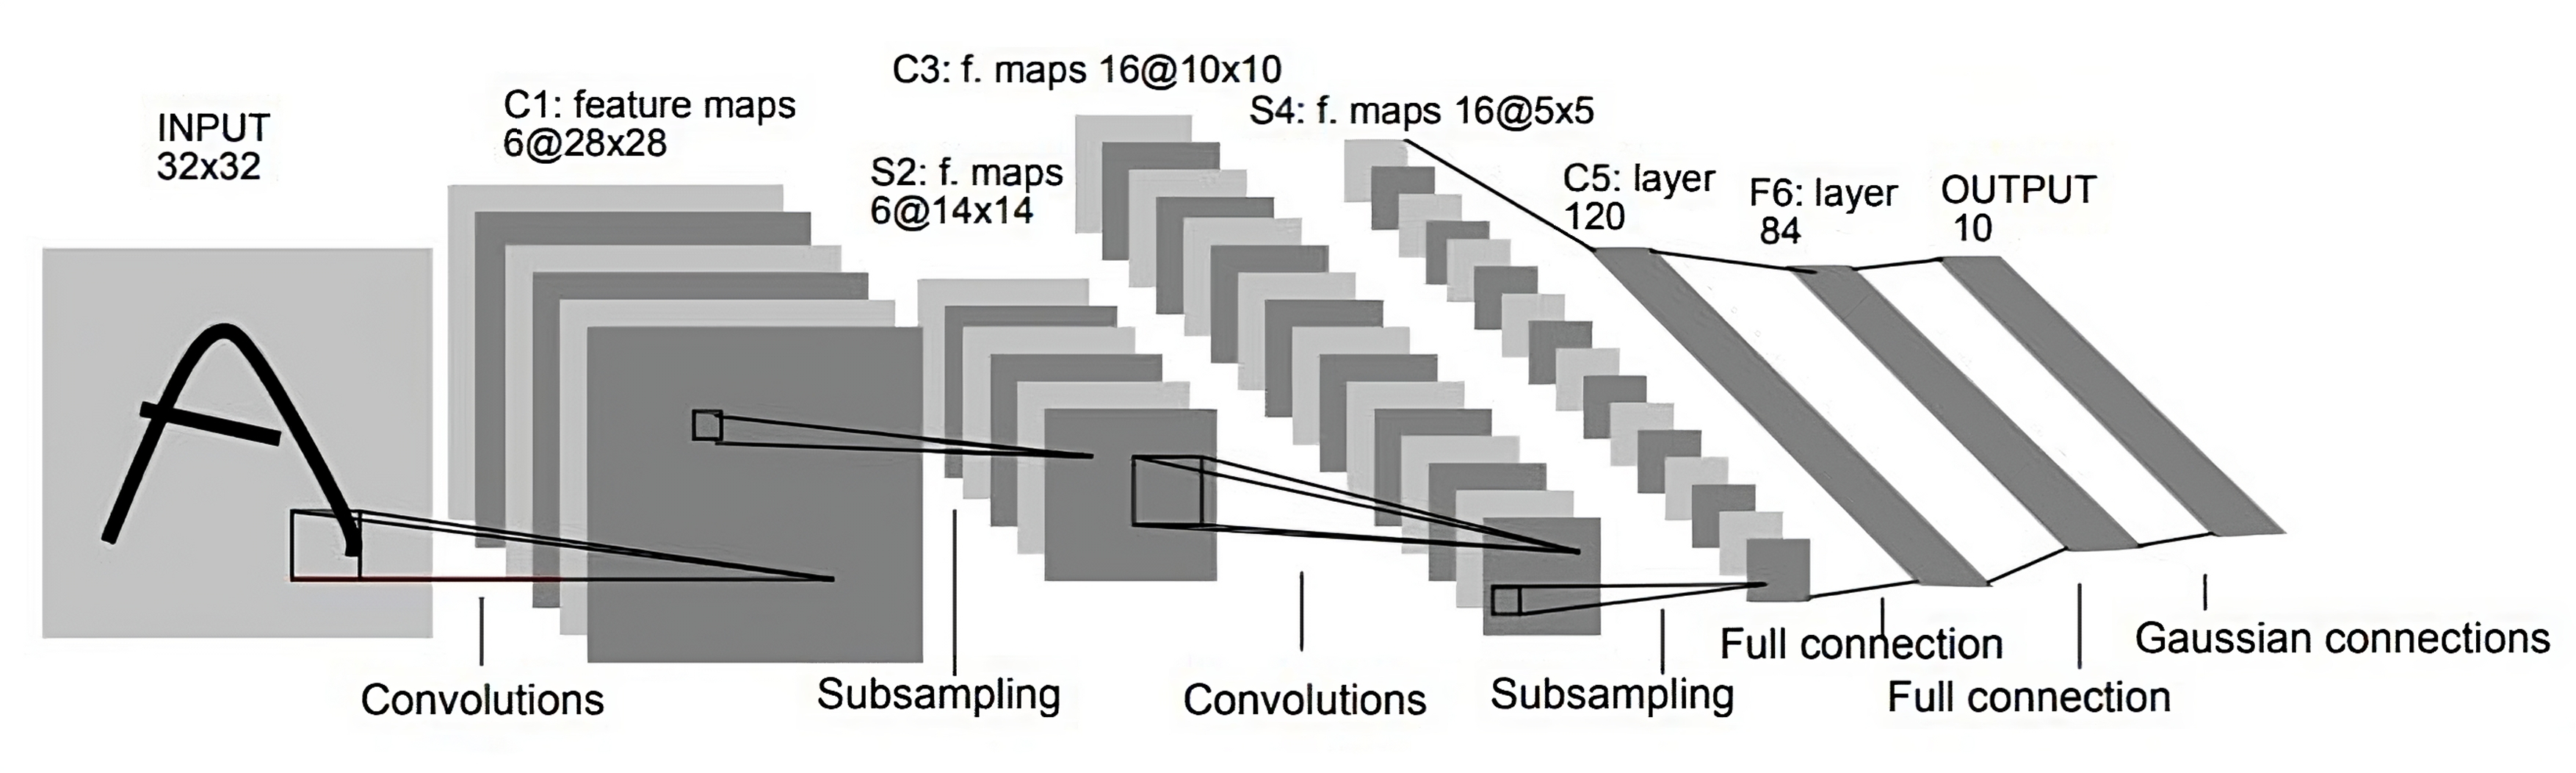
\includegraphics[width=1.2\linewidth]{images/LeNet.jpeg}}
    \caption{\gls{cnn} architecture of LeNet-5 proposed by LeCun et al. \cite{lecunGradientbasedLearningApplied1998}.}
    \label{fig:lenet}
\end{figure} 

% XAI
% ------------------------------------------
\subsection{Explainable AI (XAI)}

The rapid growth of artificial intelligence (AI) technologies has led to an increasing demand for transparency and interpretability in machine learning models. While these models have demonstrated impressive performance in various applications, their lack of transparency and interpretability has raised concerns about their reliability, accountability, and potential biases. As a result, the field of explainable AI (XAI) has emerged to address these challenges by developing techniques and tools that enable humans to understand how AI systems work and make decisions.

Explainable AI is an interdisciplinary research field that aims to make AI models more transparent, interpretable, and accountable to human users. It combines techniques from machine learning, human-computer interaction, cognitive science, and other related disciplines to develop methods and tools for explaining the behavior and decisions of AI models. The need for explainable AI arises from the fact that many machine learning models, especially deep neural networks, are often viewed as black boxes, meaning that their internal workings and decision-making processes are intricate for humans to comprehend. As a result, these models' lack of transparency and interpretability can create distrust among users, limit their adoption, and raise ethical concerns, especially in high-stakes applications such as healthcare, finance, and criminal justice.

An overview of influential methods proposed in \gls{xai} is presented in this subsection.

% LIME
\paragraph{LIME\\}
In pursuing a method that helps the explaining model to be locally faithful to the underlying model, Ribeiro et al. \cite{ribeiroWhyShouldTrust2016} proposed \gls{lime}. This model-agnostic method explains any method by learning an interpretable, less complex model locally around a specific prediction. This approach assures that the explanation is locally accurate and represents the actual inner workings of the model. 
In the same paper, they also introduce a method for explaining the global attributes of the model by framing the task as a submodular optimization problem. The technique is called SP-LIME (Submodular Pick LIME). With this approach, they can achieve global explanations that are locally accurate and faithful to the underlying model in a non-redundant way. LIME will be used later in this thesis as an explanation method adapted to a \gls{llm}.

% SHAP
\paragraph{SHAP\\}
Making non-redundant explanation features faithfully and efficiently is not easy. Lundberg et al. \cite{lundbergUnifiedApproachInterpreting2017} proposed a unified framework for interpreting predictions made by the underlying method. This framework called \gls{shap}, assigns each feature a value of importance for a specific prediction. The framework utilizes the class of additive feature attribution methods and estimates the Shapley % cite
values from cooperative game theory for that prediction. With this approach, they achieve more effective explanations to compute and have better consistency with human intuition than previously proposed methods.  


% Grad-CAM
\paragraph{Grad-CAM\\}
Visually explaining features that contributed to an image prediction can be essential in gaining trust in a model. Selvaraju et al. \cite{selvarajuGradCAMVisualExplanations2020} proposed a technique for making \glspl{cnn} more explainable and transparent by producing visual explanations for the underlying model. The method is called \gls{gradcam}, a generalization of CAM proposed by Zhou et al. \cite{zhouLearningDeepFeatures2016}, and uses the gradients in a single backtrack of any target concept. Therefore it does not need any architectural changes or retraining of the underlying prediction model to produce a localization map highlighting the crucial regions in the image for predicting the given concept, often called a saliency map in computer vision.

% DenseCap


% FLEX
\paragraph{FLEX\\}
While visual-only explanations can give the user insight into which areas of the image were essential in making the decision, they tell little to nothing about why those regions were important. On the other hand, linguistic descriptions give the user an essential understanding of the model's evaluation when predicting. 
Wickramanayake et al. \cite{wickramanayakeFLEXFaithfulLinguistic2019} propose \gls{flex} to merge saliency maps with locally accurate linguistic descriptions. In this approach, they look at the gradients through layers and identify the most critical activations in the single decision. The advantage of looking at different layers is that alongside getting an explanation that is faithful to the underlying model, they also extract features the \gls{cnn} identifies at each layer. A \gls{cnn} may represent high-level concepts, like a "car", at the last layer while identifying features such as texture and color at earlier layers. Using the activations at all essential layers, \gls{lime} achieves an image caption that explains all the essential parts of the prediction using sentences. \gls{flex} maps words to neurons in the \gls{cnn} by looking at high activations of that neuron combined with a word from the caption during the training. For this, they are using a \gls{cnn} and two stacked \gls{lstm} \cite{hochreiterLongShorttermMemory1997} cells.
The \gls{flex} framework is used as a basis for one of the two proposed methods in this thesis. A more detailed description of the specific implementation for this work is discussed later in Chapter \ref{sec3:flex_vqa}.

% VQA dataset
\paragraph{Visual Question and Answering (VQA)\\}
In order to make the linguistic abilities of computers more robust, Agrawal et al. \cite{agrawalVQAVisualQuestion2016} proposed a new dataset called \gls{vqa}. This dataset provides images from the COCO dataset \cite{linMicrosoftCOCOCommon2015}, paired with free-form, open-ended questions and answers corresponding to the content of the images. These questions and answers target different areas of the images, including underlying context and background details. This dataset aims to make models that can learn multi-modal visual and linguistic domain knowledge to get a more general and complete understanding of the world. Models that have done well in this dataset are frequently made up of \glspl{cnn}, to acquire the visual knowledge, combined with an \gls{rnn} % cite
for linguistic understanding.

Even though \gls{vqa} is not strictly \gls{xai}, it is still relevant regarding transparency to the user. \gls{vqa} is an important research area because it provides AI systems with human-readable explanations of their decision-making processes.
By providing a natural language explanation of why a specific answer was generated for a particular question about an image, \gls{vqa} models can help improve \gls{ai} systems' transparency and interpretability. This can be particularly important in domains such as healthcare and finance, where trust and transparency are critical for ensuring that \gls{ai} systems are making reliable and safe decisions. Therefore, it is important to continue developing and improving \gls{vqa} models to provide accurate and interpretable answers to questions regarding images.
Both the methods implemented and investigated in this work will be based on \gls{vqa}, using text to describe the contents of images utilizing different approaches.

\subsection{Large Language Models (LLMs)}

    \glspl{llm} are neural networks with billions or more parameters trained by self-supervised or semi-supervised learning on large amounts of text. They originated around 2018 and have performed competently on a variety of tasks. \glspl{llm} are typically general-purpose models that excel in various roles, with their performance and range of capabilities depending on the number of resources devoted during training. These models demonstrate considerable general knowledge about the world and can learn associations that make the model "memorize" numerous facts and contexts during training. 

    
    
    \glspl{llm} are pre-trained on large text datasets and can be characterized by four parameters: the size of the model, the size of the training dataset, the training cost, and the post-training performance. These variables are related by simple statistical laws called scaling laws. 

    \glspl{llm} serve not only to teach \glspl{ai} human languages but to understand proteins, write software code, and help students. These models are trained with vast amounts of text fed into the AI algorithm through unsupervised learning, allowing the model to find valuable connections in the language. Through this method, a \gls{llm} learns words, their relationships, and the concepts behind them. Large language models can also be tailored for specific use cases, including through techniques such as fine-tuning or prompt tuning, which feed the model small bits of data that must be focused on to train it for a specific application.
    
    
    However, a disadvantage of \glspl{llm} is that they can suffer from a phenomenon called hallucinations. Generative models can hallucinate because they contain vast amounts of data and organize the information in an unsupervised way. These models tend to make self-confident claims about facts not justified by their training data, which appears plausible but is not factually correct. Because of their size, they can also be challenging and computationally expensive to interpret. An ethical concern about the size of these models is that they are also computationally intensive during training and inference since they are trained on large datasets. As a result, these models have a larger carbon footprint than smaller models. However, there are ways to make these models smaller and faster, which are discussed in this chapter and also provide an overview of the development of large language models.

   

    \paragraph{BERT\\}

    BERT (Bidirectional Encoder Representations from Transformers) is a large-scale neural language model that has made significant contributions to the field of natural language processing (NLP) \cite{devlinBERTPretrainingDeep2019}. BERT is a pre-trained model that uses a transformer-based architecture that has grown in popularity in recent years due to its success in several NLP tasks. Introduced by Google in 2018, BERT is trained on a large corpus of text using an unsupervised learning approach. The model is pre-trained on a task called Masked Language Modeling (MLM), in which a small percentage of the words in a sentence are masked randomly, and the model is trained to predict the original word based on the context of the sentence. This method can be viewed as a "fill in the blanks" task, often called a cloze test, of the training sentences, keeping some words invisible to the model during training and helping the model generalize to new and unseen data. In addition, BERT is trained on an NSP task (Next Sentence Prediction), similar to the GPT models. The model is given pairs of sentences and asked to predict whether the second sentence continues the first.

    The main innovation of BERT is its ability to understand the context and provide contextualized word embeddings. Unlike previous word embeddings, which were static and did not change based on the context of the sentence, BERT can offer different embeddings to the same word depending on its context.
    
    
    
    \paragraph{BART\\}
    Lewis et al. at Facebook presented an \glspl{llm} named BART (Bidirectional and Auto-Regressive Transformer) \cite{lewisBARTDenoisingSequencetoSequence2019}. Like BERT, it uses a transformer-based architecture and is trained on a large corpus of natural language. However, unlike BERT, BART is unique because it integrates a bidirectional and auto-regressive architecture, which makes it well-suited for text generation and summarization tasks. 
    This model is a pre-trained sequence-to-sequence model that can be fine-tuned for various natural language processing tasks. BART is designed to handle auto-regressive, non-auto-regressive, generation, and comprehension tasks. The model is pre-trained on a large corpus of text using a denoising autoencoder objective, which requires the model to reconstruct original text from corrupted versions. Using a denoising autoencoder in pre-training helps reduce hallucinations by training the model to distinguish between real and fake input. 
    The authors demonstrate that BART outperforms several state-of-the-art models on various natural language generation and comprehension tasks, including summarization, question answering, and text classification. They also show that BART can be fine-tuned with relatively little data and can generalize to new domains. 
    However, instead of using Masked Language Modeling and Next Sentence Prediction like BERT, BART is pre-trained using a denoising autoencoder (DAE) objective.

    The DAE objective involves corrupting an input sequence by randomly deleting or swapping tokens and training the model to reconstruct the original sequence. This approach allows BART to handle more complex tasks such as text summarization, sentence generation, and machine translation.
        
    
    
    \paragraph{GPT\\}
    GPT (Generative Pre-trained Transformer) is a set of \glspl{llm} developed by OpenAI \cite{radfordImprovingLanguageUnderstanding2018}. Like BERT and BART, GPT is a transformer-based model but uses only an autoregressive architecture. It is pre-trained on large datasets and tuned for specific tasks. When GPT-2 was released, it was trained on a much larger dataset with significantly more parameters than GPT-1 \cite{radfordLanguageModelsAre2019}. This allowed it to generate more coherent and realistic text than its predecessor. GPT-3 is the third model in the GPT series and was released by OpenAI in 2020. It was trained on an even larger dataset than GPT-2 and had even more parameters, making it one of the largest language models. GPT-3 could generate even more readable and human-like text than its predecessors and perform various NLP tasks without explicit training \cite{brownLanguageModelsAre2020}. At the time of writing, the last published GPT model was GPT-4, which is still an autoregressive model but also includes multimodality \cite{openaiGPT4TechnicalReport2023} by making it able to interpret images. To reduce the effects of hallucinations on a generated output, GPT implements a combination of methods such as filtering and sampling.
    
    These models have proven to be versatile and powerful tools for natural language processing. GPT models have significantly influenced the NLP field, and many researchers and developers have used it as a starting point for their projects. Fine-tuned chatbot versions of GPT-3 and GPT-4 have been made available for public interaction under the name ChatGPT \cite{ChatGPT}.

    
    
    
    
    % LLaMA
    \paragraph{LLaMA\\}
    The \gls{ai} department of Meta, previously Facebook, released a modified architecture for a \gls{llm} called \gls{llama} \cite{touvronLLaMAOpenEfficient2023}.
    %This model with corresponding weights was not released to the public, but after a leak, \cite{vincentMetaPowerfulAI2023}, both the model and its weights became available to the public. 
    These models are created to compare to other \glspl{llm}, such as GPT-3 \cite{brownLanguageModelsAre2020}, Chinchilla \cite{hoffmannTrainingComputeOptimalLarge2022}, or PaLM \cite{chowdheryPaLMScalingLanguage2022}, while keeping the number of parameters considerably smaller. In the paper where Hoffman et al. propose the Chinchilla model, they also present insight into how models scale the best in conjunction with the size of the available dataset. The authors of \gls{llama} use this insight to make the model with fewer parameters perform well by training it on more tokens. The dataset that the \gls{llama} model is pre-trained on is publicly available and disclosed, which makes it compatible with open-source. The architecture is based on the transformer \cite{vaswaniAttentionAllYou2017}, with various improvements inspired by other \glspl{llm}. Some of these improvements are pre-normalization, inspired by GPT-3 \cite{brownLanguageModelsAre2020}, which improves the training stability by normalizing the input of each transformer sub-layer instead of the output. Like the PaLM model, they also use a SwiGLU as the activation function, first introduced by Shazeer at Google \cite{shazeerGLUVariantsImprove2020}, instead of ReLU. Shazeer showed it to improve the perplexities of transformer-based models. To make the self-attention mechanisms in the transformer position-agnostic, the authors implement a method called Rotary Position Embedding (RoPE) introduced by Su et al. This method allows both flexibilities of sequence length and faster convergence in fine-tuning compared to normal self-attention. With the 13 billion parameter version of \gls{llama}, the authors show that this model outperforms the GPT-3, with 175 billion parameters, on several evaluation metrics. Because the \gls{llama} model is ten times smaller than GPT-3, it can also be run on a single \gls{gpu}. These steps towards smaller, capable models benefit both the carbon footprint and inference compute budget and permit democratizing \glspl{llm} by making a model that can run on consumer hardware.

    \paragraph{Alpaca\\}
    The work in this thesis uses this Alpaca model to interpret images. More of how this model is implemented is discussed later in Chapter \ref{sec3:alpaca_vqa}.
    
    With Taori et al., Stanford University released an open-source fork of this \gls{llama} model, with some modifications, called Alpaca \cite{taoriStanfordCRFM, taoriStanfordAlpacaInstructionfollowing2023}. The Alpaca model is a fine-tuned model, with a 7B \gls{llama} model as the base model, trained on 52 thousand instruction-following tasks generated by OpenAI's text-DaVinci-003 model \cite{OpenAIAPI} using techniques from the Self-Instruct paper proposed by Wang et al. \cite{wangSelfInstructAligningLanguage2022}. Figure \ref{fig:alpaca_training} shows an overview of the Alpaca training procedure and how the dataset was built. By using text-DaVinci-003 to generate instructions, the team was able to train the model and generate the dataset for a significant cost reduction compared to traditional methods, totaling only \$600, with \$500 using OpenAI API to create the dataset and \$100 to rent 3 hours on 8 Nvidia 80GB A100 GPU cards. Reducing the cost of training an \gls{llm}, comparable to models much more expensive to develop, helps democratize these models and make them available to more people for less cost and energy.

    
    To address the ethical issue of not knowing whether a text is generated by an \gls{ai}, the team also implemented the method proposed by Kirchenbauer et al. \cite{kirchenbauerWatermarkLargeLanguage2023}. This method embeds "green" or marked tokens into the generated text, which are invisible to humans but can be detected by an algorithm analyzing a short span of these tokens.  
    The authors argue that the watermark can be embedded with negligible impact on text quality and can be detected with an efficient open-source algorithm without access to the language model API or parameters. The watermark works by choosing a random set of green tokens before generating a word and using a soft watermarking rule to encourage the input of green tokens during sampling. The authors propose a statistical test to detect the watermark with interpretable p-values and derive an information-theoretic framework to analyze the sensitivity of the watermark.

    Given the need for less computational resources, giving the method a reduced carbon footprint, and the ability to disclose the generated text as computer-generated, the Alpaca model represents a favorably ethical and transparent option for users of a system compared to other \gls{llm}. As such, it is an appropriate choice as a starting point for this thesis. This model has many of the benefits that \glspl{llm} can provide, like knowledge of vasts amount of data, while still being able to customize it to a specific task through fine-tuning. This process enables the model to adapt to a particular assignment while retaining the knowledge acquired from its initial training data.

    
    % Data flow
    \begin{figure}[htb]
        \centerline{
        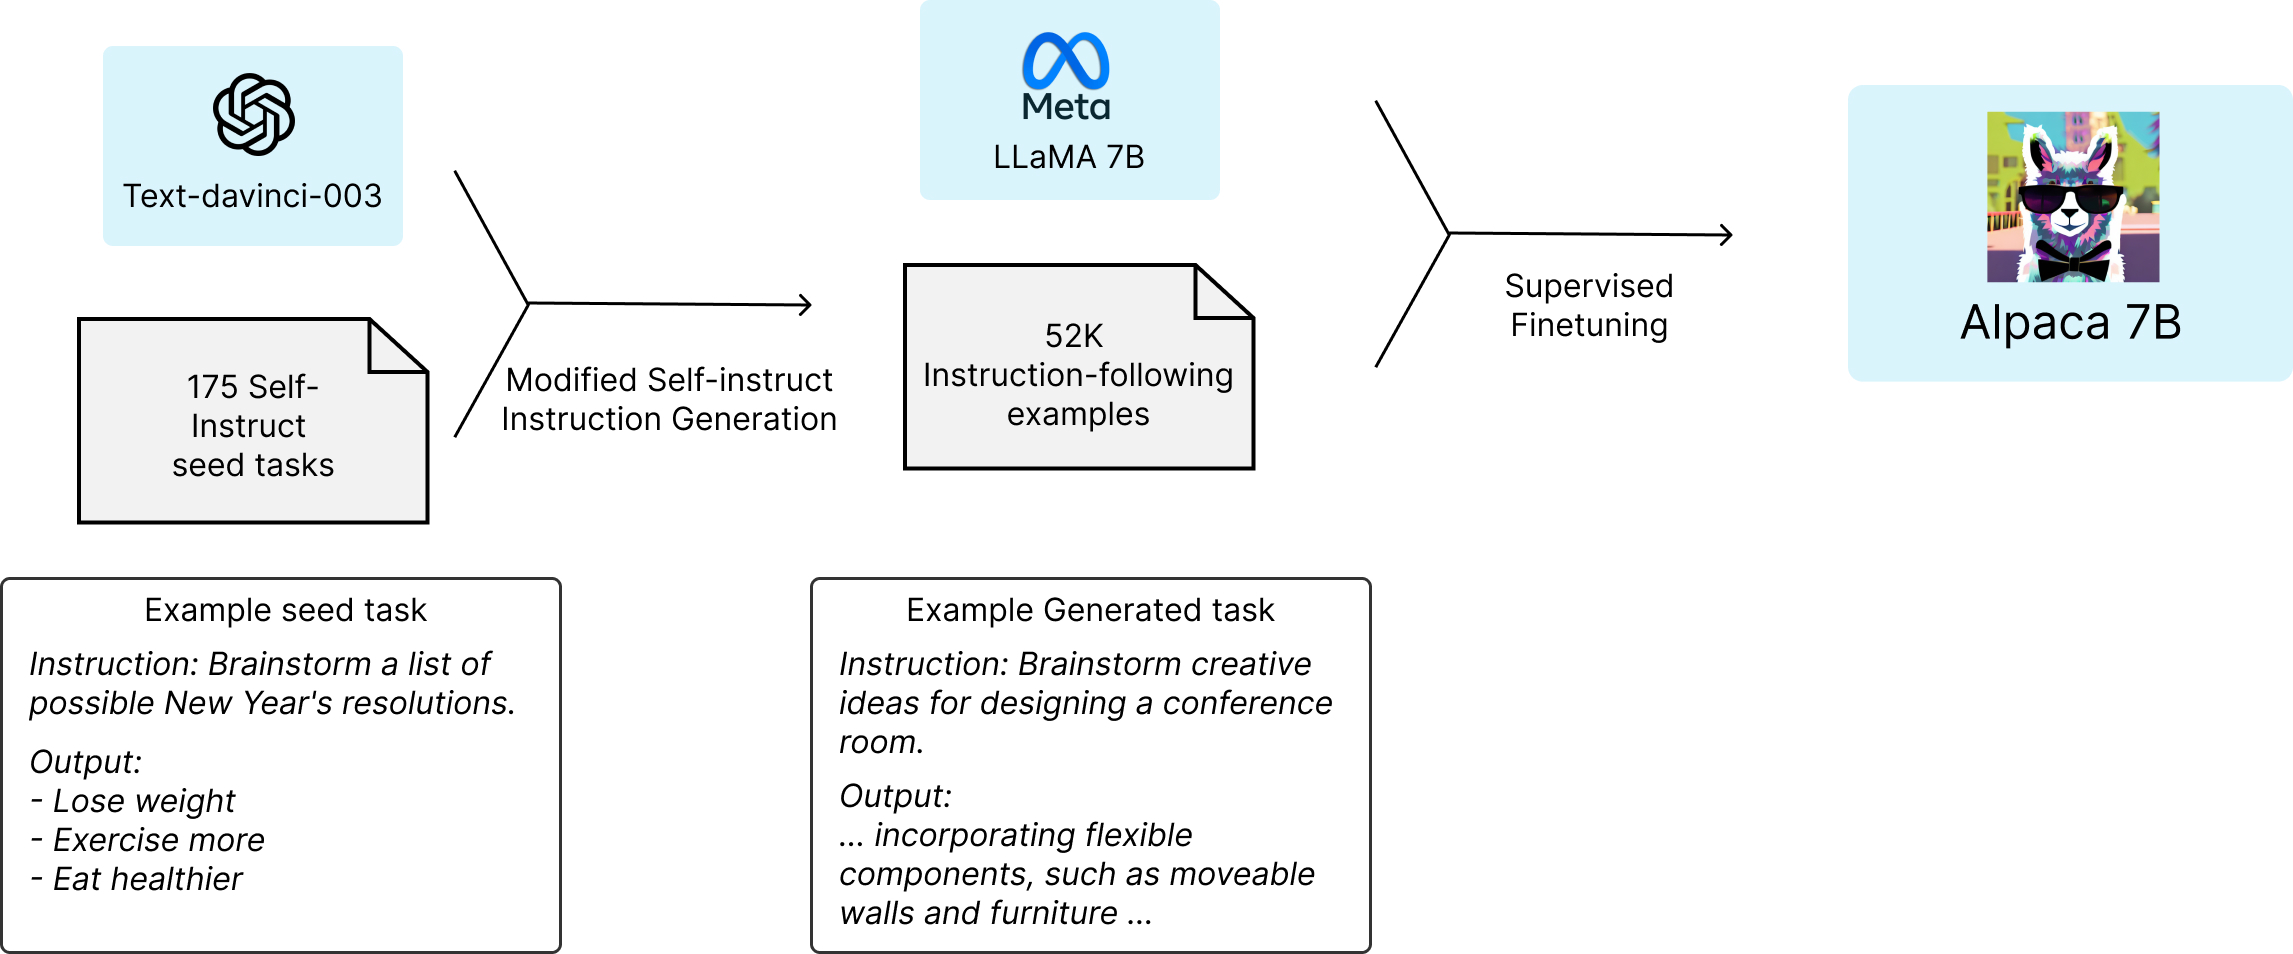
\includegraphics[width=17cm]{images/alpaca_framework.jpeg}}
        \caption[Overview of the Stanford Alpaca training procedure.]{Overview of the Stanford Alpaca training procedure.\\Figure credits: Taori et al. \cite{taoriStanfordCRFM}}
        \label{fig:alpaca_training}
    \end{figure}

%\section{Problem statement} % One page + figure?
\label{sec:1_2_problem_statement}

\begin{comment}
In a short and precise way, state what your research is about in this thesis. It can be in the form of a (set of) research questions, goals/aims, or objectives (or a mix) - but it should clearly state what the problems or challenges you are addressing.

Alternatively, one can state a research hypothesis, but if so, it should follow the rules of what a hypothesis is. A hypothesis is a statement that introduces a research question and proposes an expected result. It is an integral part of the scientific method that forms the basis of scientific experiments. Therefore, you need to be careful and thorough when building your hypothesis, following the “rules”.
\end{comment}

\section{Problem statement}

% Intro
For machine learning and computer vision to be truly trustworthy, they will need to be understood. Researchers need to understand the inner workings of the model to improve it and discover biases in the dataset. Users and domain experts utilizing the models need to have trust in the model predicting accurately while using useful features when evaluating. The models should be able to achieve \gls{sota} performance, without sacrificing interpretability and explainability in what they evaluate when predicting. 

% What this is and How I want to do it
In this thesis, the goal is to explore the roam of visual and linguistic understanding.
The visual knowledge will come from a \gls{cnn} that learns features in images. An \gls{rnn} \cite{rumelhartLearningRepresentationsBackpropagating1986, choLearningPhraseRepresentations2014, sutskeverSequenceSequenceLearning2014, bahdanauNeuralMachineTranslation2016} or transformer is used to extract linguistic information from open-ended questions and answers in natural language, taken from a \gls{vqa} dataset. A backward pass that looks for large gradients through layers of the \gls{cnn} will be used to choose locally faithful words to caption the image in an explainable way. 



% Questions to be answered
The main topics that will be explored to reach the research goal are: 
\begin{itemize}
    \item Does an explainable image caption model improve its answers when trained on a \gls{vqa} dataset?
    \item With only the explaining model choosing the captions, will the output be more intuitive for humans?
    \item Are the explanations, both captions, and answers from open-ended questions locally faithful to the underlying \gls{cnn} model?
    \item If there is enough time during this thesis, it would be an interesting task to see if the image caption and \gls{vqa} will perform better when using transfer learning  on a language model pretrained on a large language dataset. 
\end{itemize}

% What is the result
With these research questions answered, this thesis will be one step closer to an explanatory model that can give insight into how models understand broad concepts in vision and language. This knowledge can be used to make computers understand a more complex worldview and help humans understand what it sees and value.

\subsection{Proposed architecture}
Figure \ref{fig:architecture_proposal} shows how the data flow in the proposed method can work. It closely follows the \gls{flex} \cite{wickramanayakeFLEXFaithfulLinguistic2019} architecture proposed by Wickramanayake et al. It consists of a \gls{cnn} that extracts visual information and a 2-layered \gls{lstm} \cite{hochreiterLongShorttermMemory1997} \gls{rnn} that combine linguistic information with extracted visual features. The reason why this architecture is relevant for this thesis is that it uses a backward pass to find locally accurate visual features, which are then used to give an image caption that describes what visual features actually were important to the classification and captioning of the image. This makes the architecture useful as a starting point for this thesis and can be adapted to use \gls{vqa} datasets as linguistic input, to make it possible to ask questions regarding the classification of images and predictions. 

% Explain the proposed data flow / architecture 
    % Training
    % CNN
During training the proposed architecture takes an image and its corresponding questions and answers from the \gls{vqa} dataset. The images are fed through a \gls{cnn}-network, which can be pretrained on a larger dataset, like ImageNet \cite{dengImageNetLargeScaleHierarchical2009}. This is because the explaining method utilizes feature maps in each layer of the \gls{cnn}, so it is agnostic on what type of \gls{cnn} it is and what dataset it is trained on earlier. The \gls{cnn} predicts a class of what it sees in the image, and with a backward pass, finds important feature maps in each  convolutional layer. Each feature in the set of important feature maps gets associated with a word and stored in a relevance vector. This process is done by computing a co-occurrence score between each word in the ground truth caption and the feature. The feature with the highest co-occurrence score gets linked with that feature. 

    % LSTM
The \glspl{lstm} gets trained by feeding each word in the ground truth caption into the first layer, alongside the hidden state of the \gls{lstm}. This is used to compute the next state, which gets concatenated with important visual features, and is input to the second, and last, \gls{lstm}-layer. 
The output from the second \gls{lstm}-layer is encoded to vocabulary space that is used to make a conditional probability distribution that later will be used to calculate the probability for predicting that word, given the given image features. 

    % Testing
During prediction, the architecture takes an image and an optional question as input. The \gls{cnn} extracts important features in the layers, which get fed into the \gls{lstm}. Important feature maps from the \gls{cnn} are also used to calculate the relevance vector between features in the image and words. The \gls{lstm} uses this relevance vector, alongside important decision-relevant features from the image to predict a word. This word prediction is repeated until the stop word is predicted. 

If no question is input to the algorithm during prediction, the model will use the most accurate predicted answer caption that describe the image as a whole as a caption for the image. On the other hand, if a question is submitted alongside the image, the \gls{lstm} will generate captions that answer the question asked, and then choose the most decision-relevant answer as the caption. 



% Data flow
\begin{figure}[htb]
    \centering
    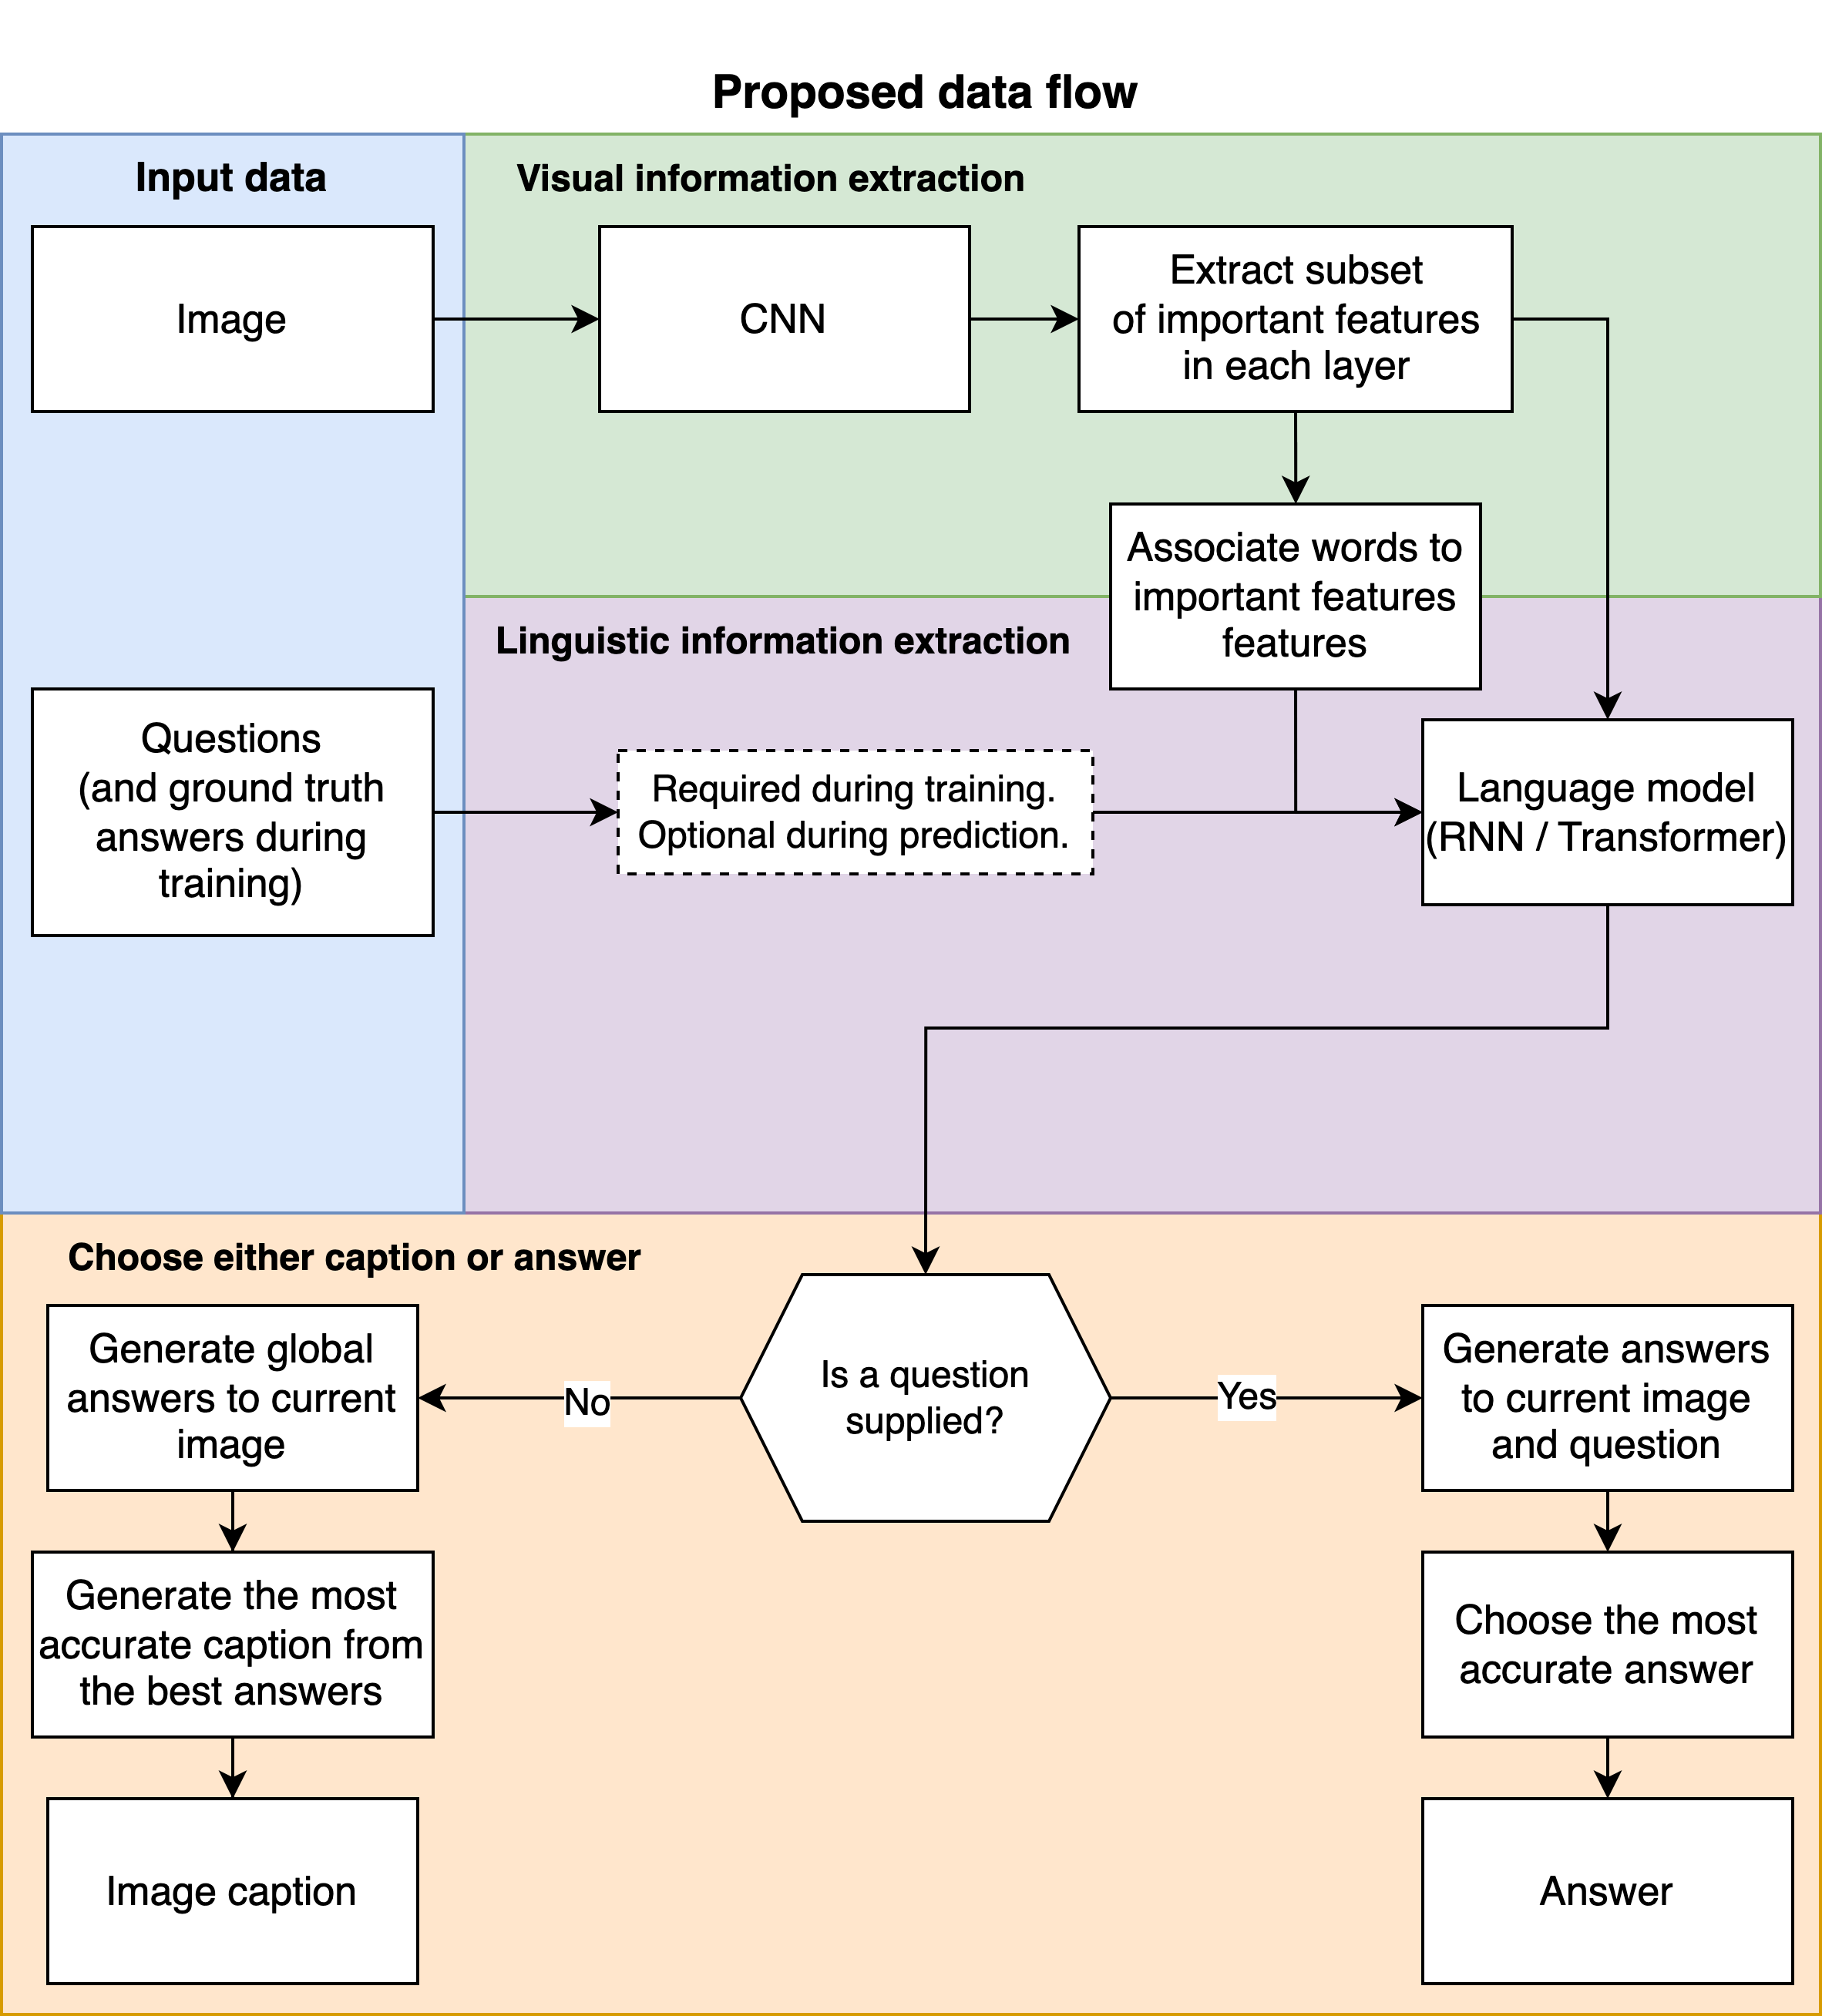
\includegraphics[width=12cm]{images/architecture_proposal.png}
    \caption{Proposal of the data flow and components that will be explored in this thesis.}
    \label{fig:architecture_proposal}
\end{figure}


%\backmatter{}
\newpage
\printbibliography
\end{document}
